\iffalse
\documentclass[12pt]{article}
\usepackage{graphicx}
%\documentclass[journal,12pt,twocolumn]{IEEEtran}
\usepackage[none]{hyphenat}
\usepackage{graphicx}
\usepackage{listings}
\usepackage[english]{babel}
\usepackage{graphicx}
\usepackage{caption} 
\usepackage{hyperref}
\usepackage{booktabs}
\usepackage{commath}
\usepackage{gensymb}
\usepackage{array}
\usepackage{amsmath}   % for having text in math mode
\usepackage{listings}
\lstset{
  frame=single,
  breaklines=true
}
  
%Following 2 lines were added to remove the blank page at the beginning
\usepackage{atbegshi}% http://ctan.org/pkg/atbegshi
\AtBeginDocument{\AtBeginShipoutNext{\AtBeginShipoutDiscard}}
%


%New macro definitions
\newcommand{\mydet}[1]{\ensuremath{\begin{vmatrix}#1\end{vmatrix}}}
\providecommand{\brak}[1]{\ensuremath{\left(#1\right)}}
\providecommand{\norm}[1]{\left\lVert#1\right\rVert}
\newcommand{\solution}{\noindent \textbf{Solution: }}
\newcommand{\myvec}[1]{\ensuremath{\begin{pmatrix}#1\end{pmatrix}}}
\let\vec\mathbf
\begin{document}
\begin{center}
\title{\textbf{Circles}}
\date{\vspace{-5ex}} %Not to print date automatically
\maketitle
\end{center}
\setcounter{page}{1}
\section{11$^{th}$ Maths - Exercise 11.1.9}

\begin{enumerate}
\item Find the centre and radius of the given circle $2x^2+2y^2-x=0$
\section{Solution}
\fi
The given equation can be expressed as 
\begin{align}
	x^2+y^2-\frac{x}{2}&=0
	\\
\implies 	\norm{\vec{x}}^2+2\myvec{\frac{-1}{4} & 0}\vec{x}&=0
\end{align}	
The centre of circle is then given by 
\begin{align}
	\vec{u} = -\vec{c} 
=\myvec{\frac{1}{4}\\0}
\end{align}
and the radius of circle is obtained as
\begin{align}
	r=\sqrt{\norm{\vec{u}}^2 -f}
=\frac{1}{4}
\end{align}
See Fig. 
  \ref{fig:chapters/11/11/1/9/Figure}.
\begin{figure}[h]
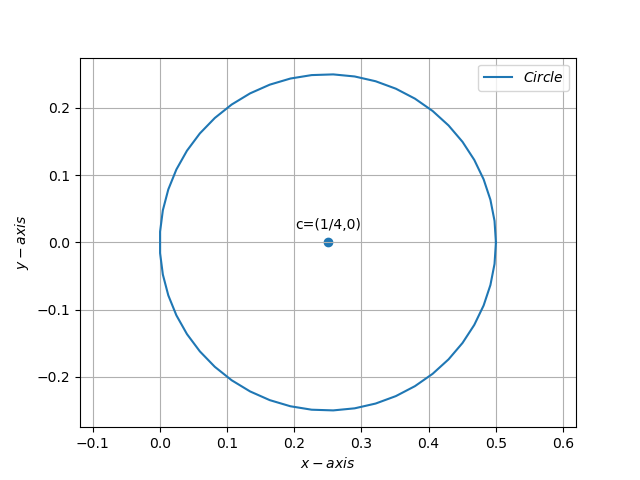
\includegraphics[width=\columnwidth]{chapters/11/11/1/9/figs/fig.png}
\caption{}
  \label{fig:chapters/11/11/1/9/Figure}
\end{figure}
